% 第 6 题点列图：按固定源 PDF 矢量路径换算（1 pt → 0.03515 cm）。
% 原点取下边射线的左端（源页 (155.6289, 652.3750) pt），y 向上。
% 两条截断射线（角顶点在图外，源图有意不画）；三个浅灰填充三角形 S1/S2/Sn；
% 点列 A1..A(n+1) 在上射线、B1..B(n+1) 在下水平线（等距 20.22 pt）；16 组文字标签。
% 注：两射线已画端点纵向相距 23.05 pt、横向错开仅 0.40 pt（被同一竖直截断线切齐），
% 判为有意截断（交点外推约 (114.5, 652.4)），照源复刻不补顶点。
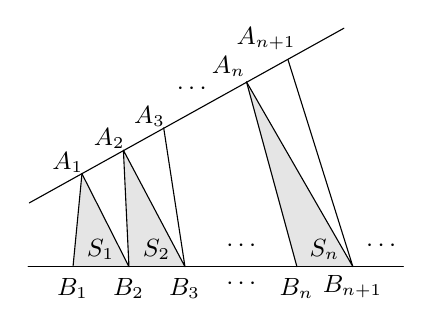
\begin{tikzpicture}[line cap=round,line join=round,font=\small,x=0.03515cm,y=0.03515cm]
% ===== 浅灰填充三角形（fill-opacity 0.1）=====
\fill[black,fill opacity=0.1] (19.41,33.57)--(16.18,0)--(36.39,0)--cycle;
\fill[black,fill opacity=0.1] (34.38,42.06)--(56.62,0)--(36.39,0)--cycle;
\fill[black,fill opacity=0.1] (78.86,66.73)--(97.06,0)--(117.28,0)--cycle;
% ===== 线画 =====
\draw (135.48,0)--(0,0);                 % 下边（水平射线，B 点列所在）
\draw (114.04,86.14)--(0.40,23.05);      % 上边（斜射线，A 点列所在）
\draw (19.41,33.57)--(16.18,0);          % A1B1
\draw (19.41,33.57)--(36.39,0)--(34.38,42.06)--(56.62,0)--(48.93,50.15);  % A1→B2→A2→B3→A3
\draw (78.86,66.73)--(97.06,0);          % AnBn
\draw (78.86,66.73)--(117.28,0)--(93.82,74.82);  % An→Bn+1→An+1
% ===== 文字标签（照源字形框中心，显式坐标）=====
\node[anchor=center,inner sep=0] at (14.30,37.75) {\(A_{1}\)};
\node[anchor=center,inner sep=0] at (29.27,46.25) {\(A_{2}\)};
\node[anchor=center,inner sep=0] at (43.83,54.34) {\(A_{3}\)};
\node[anchor=center,inner sep=0] at (59.05,64.27) {\(\cdots\)};
\node[anchor=center,inner sep=0] at (72.36,72.33) {\(A_{n}\)};
\node[anchor=center,inner sep=0] at (85.92,82.25) {\(A_{n+1}\)};
\node[anchor=center,inner sep=0] at (26.11,6.21) {\(S_{1}\)};
\node[anchor=center,inner sep=0] at (46.34,6.21) {\(S_{2}\)};
\node[anchor=center,inner sep=0] at (76.93,7.65) {\(\cdots\)};
\node[anchor=center,inner sep=0] at (107.02,6.21) {\(S_{n}\)};
\node[anchor=center,inner sep=0] at (127.50,7.65) {\(\cdots\)};
\node[anchor=center,inner sep=0] at (15.99,-7.74) {\(B_{1}\)};
\node[anchor=center,inner sep=0] at (36.22,-7.74) {\(B_{2}\)};
\node[anchor=center,inner sep=0] at (56.45,-7.74) {\(B_{3}\)};
\node[anchor=center,inner sep=0] at (76.93,-6.30) {\(\cdots\)};
\node[anchor=center,inner sep=0] at (96.91,-7.74) {\(B_{n}\)};
\node[anchor=center,inner sep=0] at (117.13,-7.32) {\(B_{n+1}\)};
\end{tikzpicture}
